\documentclass[IN,11pt,twoside,openright,master,english]{tumthesis}

% Include common packages
\usepackage{packages/packages}
\usepackage{listings}
\usepackage{xr}
\externaldocument{include/bibliography}

\graphicspath{ {./images/} }


% IEEE tools for tweaking bib style
\usepackage{IEEEtrantools}

\newcommand\toc{\relax}

\usepackage[backend=bibtex,style=ieee]{biblatex}
\usepackage{booktabs}
\usepackage{tabularx}
\usepackage{longtable}
\usepackage{tabu}
\usepackage{ltxtable}
\usepackage{url}
\usepackage[style=base]{caption}
\captionsetup{%
	font={rm,footnotesize},
	labelfont={sc},
}
\captionsetup[subfloat]{%
	font={rm,footnotesize},
	labelfont={rm},
}
\usepackage{subfig}
\usepackage{nicefrac}
\usepackage{longtable}
\usepackage[hang]{footmisc}
\usepackage{acro}
\usepackage{blindtext}


\setlength\footnotemargin{5pt}

% Theorem environments
\newtheorem{definition}{Definition}
\newtheorem{theorem}{Theorem}
\newtheorem{example}{Example}
\newtheorem{lemma}{Lemma}


% hyphenation
\hyphenation{op-ti-cal net-work net-works semi-con-duc-tor tech-nique tech-niques}


\usepackage{mdframed}
\newlength{\charwidth}
\setlength{\charwidth}{\widthof{\scriptsize\texttt{x}}}

\makeatletter
\newenvironment{moeplstborder}[2][]{%
\ifx#1\@empty\@empty%
	\edef\@margin{-1.5\baselineskip}%
\else%
	\edef\@margin{#1}%
\fi%
\vspace{-\baselineskip}
\begin{center}
\begin{minipage}{#2}
\begin{mdframed}[%
	topline=false,leftline=false,bottomline=false,rightline=true,
	linecolor=TUMRed!20,linewidth=\charwidth,
	innertopmargin=\@margin,innerbottommargin=-0.5\baselineskip,
	innerleftmargin=0pt,innerrightmargin=-\charwidth,
	userdefinedwidth=#2,
]%
}%
{%
\end{mdframed}%
\end{minipage}
\end{center}
}%
\makeatother

% Needed for Bachelor's theses, Master's theses and IDP
\titleenglish{Efficient and Accurate Hop-by-Hop Capacity Estimation}
\titlegerman{Effiziente und Genaue Hop-by-Hop Kapazit\"atsabsch\"atzungen}
\author{Bakar Andguladze}
\supervisor{\NEThead}
\advisor{Prof.~Dr.-Ing.~Georg~Carle}
\assistants{Simon Bauer\tlc{}~M.\,Sc.,%
Benedikt~Jaeger\tlc{}~M.\,Sc.}

% in case of bachelor's/master's thesis use your own field of study
%\courseofstudy{Informatik}
\courseofstudy{Informatics}
%\courseofstudy{Informatik: Games Engineering}
%\courseofstudy{Informatics: Games Engineering}

% in case of idp use electrical engineering as your field of study
%\courseofstudy{Elektrotechnik}
%\courseofstudy{Electrical Engineering}

\date{November 15, 2021}
\location{Garching}

\setcounter{tocdepth}{2}

% Deprecated version, works for acro (< v3 and >= v3)
\acsetup{%
	list-style=longtable,
	extra-style=plain,      % remove dot after long in list
	only-used=false,
}

% No-warnings version for newer versions of acro (>= v3)
%\acsetup{%
%	list/template=longtabu,
%	list/display=all
%}

\tabulinesep=1ex

\DeclareAcronym{mss}{
	short				= {\sc{MSS}},
	long				= {Maximum Segment Size},
	list				= {\acl{mss}.},
}
\DeclareAcronym{mtu}{
	short				= {\sc{MTU}},
	long				= {Maximum Transmision Unit},
	list				= {\acl{mtu}.},
}
\DeclareAcronym{tcp}{
	short				= {\sc{TCP}},
	long				= {Transmission Control Protocol},
	list				= {\Acl{tcp}.},
	extra				= {%
		Stream-oriented, reliable, transport layer protocol.
	}
}
\DeclareAcronym{icmp}{
	short				= {\sc{ICMP}},
	long				= {Internet Control Message Protocol},
	list				= {\acl{icmp}.},
}
\DeclareAcronym{udp}{
	short				= {\sc{UDP}},
	long				= {User Datagram Protocol},
	list				= {\acl{udp}.},
	extra				= {%
		Datagram-oriented, unreliable transport layer protocol.
	}
}
\DeclareAcronym{ip}{
	short				= {\sc{IP}},
	long				= {Internet Protocol},
	list				= {\acl{ip}.}
}

\DeclareAcronym{iso}{
	short				= {\sc{ISO}},
	long				= {International Organization for Standardization},
	list				= {\acl{iso}.},
}
\DeclareAcronym{osi}{
	short				= {\sc{OSI}},
	long				= {Open Systems Interconnection},
	list				= {\acl{osi}.},
	extra				= {%
		Reference model for layered network architectures by the \ac{osi}.
	},
}

\DeclareAcronym{vps}{
	short				= {\sc{VPS}},
	long				= {Variable Packet Size},
	list				= {\acl{vps}.},
}

\DeclareAcronym{pptd}{
	short				= {\sc{PPTD}},
	long				= {Packet Pair/Train Dispersion},
	list				= {\acl{pptd}.},
}

\DeclareAcronym{rtt}{
	short				= {\sc{RTT}},
	long				= {Round Trip Time},
	list				= {\acl{rtt}.},
}

\DeclareAcronym{ttl}{
	short				= {\sc{TTL}},
	long				= {Time-To-Live},
	list				= {\acl{ttl}.},
}


\DeclareAcronym{pdu}{
	short				= {\sc{PDU}},
	short-plural-form	= {\sc*{PDU}s},
	long				= {protocol data unit},
	long-plural-form	= {protocol data units},
	list				= {\Acl{pdu}.},
	extra				= {%
	Refers to a message at a specific layer of the \acs{osi} model including
	all headers and trailers of the respective layer and all layers above.
	},
}
\DeclareAcronym{sdu}{
	short				= {\sc{SDU}},
	short-plural-form	= {\sc*{SDU}s},
	long				= {service data unit},
	long-plural-form	= {service data units},
	list				= {\Acl{sdu}.},
	extra				= {%
		Refers to the payload of a message at a specific layer of the \acs{osi}
		model excluding all headers and trailers of the respective layer.
	},
}
\DeclareAcronym{mac}{
	short				= {\sc{MAC}},
	long				= {medium access control},
	list				= {\Acl{mac}.},
}
\DeclareAcronym{sctp}{
	short				= {\sc{SCTP}},
	long				= {Stream Control Transmission Protocol},
	list				= {\acs{sctp}.},
	extra				= {%
		Datagram-oriented, semi-reliable transport layer protocol.
	}
}




\addbibresource{bib/IEEEfull.bib}
\addbibresource{bib/litnew.bib}


%\renewcommand{\andothersdelim}{}
%bib.sty does not work older bibtex versions (works on TexLive 2016 or newer)
%\usepackage{bib}

% Load late to avoid same identifier warning
\usepackage[colorlinks=false,pdfborder={0 0 0}]{hyperref}


\begin{document}%

% Makes sure that same author names are not replaced by dahes
\bstctlcite{IEEEexample:BSTcontrol}

\pagenumbering{gobble}
\maketitle%
\cleardoublepage


\begin{abstract}
	Abstract of the thesis will be written afterwards
\end{abstract}

%begin{otherlanguage}{ngerman}
%	\begin{abstract}
%		\small

\blindtext

\blindtext

%	\end{abstract}
%\end{otherlanguage}

%\begin{thanks}
%%\input{/home/moepi/.thanks}
%\end{thanks}

%\begin{preface}
%foo bar
%\end{preface}

\tableofcontents
\listoffigures
\listoftables

\startcontent

\chapter{Introduction}
This master thesis presents the capacity estimation method for hop-by-hop measurements. Our goal is to create and test a method of calculating the capacity (i.e. maximum transmission rate) in a given network path and locating the narrow link.
We will test the developed tool in regard to various metrics, such as packet size, intrusion rate, cross-traffic and flow-interference and finally, analyze the test results in order to conclude whether our approach is actually capable of delivering accurate results efficiently. 

\section{Motivation}
As the Internet is becoming increasingly essential part of our day-to-day lives, it is ever more important for the Internet providers to enhance the quality of networks in order to create a better user experience. One of the means to achieve this goal is to have a better picture of the network they aim to improve. Therefore, we are going to create a tool that measures the capacity of the path between two hosts. The intended field of application is, for instance, enhancing the performance of network, traffic analysis, network monitoring, etc. 

There are quite a few capacity estimation methodologies and tools available, that will be discussed in chapters below. However, the current State-of-the-Art methods have some significant flaws and limitations regarding our measurement goals, such as  
\begin{itemize}
	\item High intrusion, which can lead to network overload,
	\item Dependence on ongoing traffic, which can be unpredictable at times,
	\item Inability to locate the narrow link on the path.
\end{itemize}

Therefore, our goal is to develop a new solution that tries to minimize the influence of these limitations in regard to our measurement objectives. We will try to implement the least possible intrusion without compromising the accuracy. Also our tool will be able to find the first narrow link of the path by measuring the capacity of each hop in the network. 

This new solution will be tested and evaluated in comparison to the results of existing capacity measurement tools, i.e. PPrate implementation by Patryk Brzoza[x], but in contrast to Brzoza’s passive approach our tool will be based on an active measurement methodology. Moreover Brzoza’s measurement tool was designed to estimate end-to-end capacity, while this thesis is concerned about measuring the capacity of each hop in the network and finding the narrow link, as hop-by-hop measurements provide a better picture of a network and enable to take a closer look at potential issues.



\section{Research Questions}
This thesis is supposed to answer the following research questions:

\begin{itemize}
  \item \textbf{How to measure network capacity hop-by-hop?}
  \\In order to measure the path capacity hop-by-hop, we need to estimate capacities to each router on the path until the destination host is reached. 
  \item \textbf{How to optimize the trade-off between accuracy and intrusiveness regarding large-scale measurements?}
  \\Certain level of intrusion into the network will be necessary for the measurements. However there is an important factor to consider: too high intrusion could disrupt the traffic in the network and too low could lead to unreliable results. Therefore an optimal middle ground has to be found: What will be the optimal amount of packets to send to each router to get correct results?
  \item \textbf{How robust is the proposed solution regarding the handling of cross-traffic, flow-interference and sudden path parameter changes?}
  \\Real networks are usually quite complex and different challenges might arise when we are trying to measure the path capacity. We need to find out whether our solution is feasible when it faces cross-traffic, flow-interference or when the path parameters suddenly change.
  \item \textbf{Are we able to locate the capacity bottlenecks of a network?}
  \\ We are interested to find the location of the weakest link in the given network. This can be achieved by finding the capacities to each hop. The weakest link will 
\end{itemize}

\section{Outline}
This section introduces the structure of the thesis.
\\Chapter 2 defines the necessary terminology for understanding this thesis. Namely, capacity, TCP, ICMP, Raw sockets, etc. 
\\Chapter 3 describes the related work - what has been done in regard to capacity estimations and some drawbacks and limitations to the existing approaches
\\Chapter 4 describes the approach and the tool that we have developed to implement it. 
\\Chapter 5 reviews the test setup and test environment in which the experiments are conducted.
\\Chapter 6 evaluates our approach based on several parameters. It reviews the different factors that might affect the measurements and to what extent. Namely, how packet length influences the measurement results, what is the optimal rate of intrusion in the network and whether the cross-traffic and the flow-interference cause higher inaccuracy. Based on how the proposed approach handles these challenges we can state whether it is reliable or not.
\\Finally, chapter 7 concludes our thesis and subsequently discusses the future work - what can be done afterwards to further extend our methodology. 

\chapter{Background}
The following chapter provides the background information and defines the important terminology that is useful to understand our work.

\section{Terminology}
Certain terms in our area of research can be used with different meanings, therefore we first need to state that this thesis will be using the definitions provided by Prasad et al. \cite{Prasad2003} in their paper "Bandwidth estimation: metrics, measurement, techniques and tools", as it appears to be more widespread and accepted, as those are the definitions also used by other researchers at the chair, therefore, it is more practical to use the common language.

Prasad et al.\cite{Prasad2003} introduce the following three metrics: capacity, bandwidth and bulk transfer capacity(BTC), capacity being the main focus of our work.
Moreover, they distinguish between segments and hops. The former being the link at the data link layer (L2) and the latter - the links at the IP layer (L3).

% this is a copy. fix it.%%%%%%%%%%%%%%%%%%%%%%%%%%%%%%%%%%%%%%%%%%%%%%%%
[THIS IS A COPY]
A segment normally corresponds to a physical point-to-point link, a virtual circuit, or to a shared access local area network (e.g., an Ethernet collision
domain, or an FDDI ring). In contrast, a hop may consist of a sequence of one or more segments, connected through switches, bridges, or other layer-2 devices. We
define an end-to-end path from an IP host (source) to another host (sink) as the sequence of hops that connect to 
%%%%%%%%%%%%%%%%%%%%%%%%%%%%%%%%%%%%%%%%%%%%%%%%%%%%%%%%%%%%%%%%%%%%%%%%%

\subsection*{Capacity}
[ALSO COPY]
A layer-2 link, or segment, can normally transfer data at a constant bit rate, which is the transmission rate of the segment. For instance, this rate is 10Mbps
on a 10BaseT Ethernet segment, and 1.544Mbps on a T1 segment. The transmission rate of a segment is limited by both the physical bandwidth of the underlying
propagation medium as well as its electronic or optical transmitter/receiver hardware. 
At the IP layer a hop delivers a lower rate than its nominal transmission rate due to the overhead of layer-2 encapsulation and framing. Specifically, suppose that the nominal capacity of a segment is

%\Delta _{L3} = \dfrac{L_{L3}+H_{L2}}{C_{L2}}

The transmission time for an IP packet of size bytes is

\subsection*{Available Bandwidth}
Another important metric is the available bandwidth of a link or end-to-end path. The available bandwidth of a link relates to the unused, or “spare”, capacity of the link during a certain time period. So even though the capacity of a link depends on the underlying transmission technology and propagation medium, the available bandwidth of a link additionally depends on the traffic load at that link, and is typically a time-varying metric.

\section{Network Layers}

\section{TCP}
https://datatracker.ietf.org/doc/html/rfc793
header diagrams.

\section{UDP}

\section{ICMP}
\label{icmp_section}
https://datatracker.ietf.org/doc/html/rfc792

\section{Traffic Generation}

\subsection*{Raw Sockets}
https://www.binarytides.com/raw-sockets-c-code-linux/


\subsection*{iPerf}

\subsection*{Capturing Traffic}
\url{https://www.wireshark.org/docs/man-pages/tshark.html}
tcpdump

\section{Capacity Estimation}
general explanation

\subsection{End-to-End vs Hop-by-Hop Capacity Estimation}

\subsection{Active vs Passive Capacity Estimation}

\chapter{Related Work}

\section{Existing Approaches}

\subsection*{Variable Packet Size Probing}

\subsection*{Packet Pair/Train Probing}

\section{Implementation of PPrate by Brzoza}
 

\chapter{Implementation}

\section{Analysis}

\section{Approach}

\section{Traffic Generation}

\section{Estimation of End-to-End Capacity}

\section{Estimation of Capacities Hop-by-Hop}

\subsection*{parameters(?)}

\section{Locating the Narrow Link}



\chapter{Evaluation}
This chapter presents the results of the evaluation of our approach. The experiments have been conducted based on several test parameters and their combinations and we will be analyzing the baseline parameter sets as well as key combinations. 

We evaluate based on the path length, capacity range, packet size, number of packets. For the better insight we also apply artificial packet loss and icmp rate limit. 
The tests are conducted on the empty network as well as with significant amount of cross-traffic load.

The following \texttt{JSON} serves as an example of a configuration file used for experiments.
It contains default parameter values, each of which will be manipulated respectively in upcoming sections:
\begin{lstlisting}
{    
  "topo_size": 3, // path length
  "capacity_range": [10, 100],			
  "capacity_delta": 5
  "packet_size": 1400,
  "packets_per_hop": 300,
  "icmp_ratelimit": 0,
  "packet_loss": 0,
  "cross_traffic": 0.0,
  "output": "results/results.csv"
}
\end{lstlisting}

\section{Test Setup}

%%%%%%%%%%%%%%%%%%%%%%%%%%%%%%%%%%%%%%%%%%%%%%%%%%%%%%%%%%%%%%%%%%%%%%%%%%%%%%%%%
\section{Path Length}
The first parameter to be discussed is the path length from the source host to the sink. 

\subsection*{Conclusion}
We can conclude that the path length doesn't affect the accuracy of the estimation tool. After testing the 

%%%%%%%%%%%%%%%%%%%%%%%%%%%%%%%%%%%%%%%%%%%%%%%%%%%%%%%%%%%%%%%%%%%%%%%%%%%%%%%%%
\section{Packet Size}
The first and one of the key parameters in our evaluation is the packet size. 
Based on the test results we were able to observe that the optimal packet size depends on the capacity range of the network. 

\subsection*{Estimation Error}

\subsection*{Conclusion}


%%%%%%%%%%%%%%%%%%%%%%%%%%%%%%%%%%%%%%%%%%%%%%%%%%%%%%%%%%%%%%%%%%%%%%%%%%%%%%%%%
\section{Packets per Hop}

\subsection*{Conclusion}

%%%%%%%%%%%%%%%%%%%%%%%%%%%%%%%%%%%%%%%%%%%%%%%%%%%%%%%%%%%%%%%%%%%%%%%%%%%%%%%%%
\section{Cross-Traffic}
Cross traffic seems to affect the test results significantly. 
What does 1.0 mean?

\subsection*{Conclusion}

%%%%%%%%%%%%%%%%%%%%%%%%%%%%%%%%%%%%%%%%%%%%%%%%%%%%%%%%%%%%%%%%%%%%%%%%%%%%%%%%%
\section{Packet Loss}

\subsection*{Conclusion}

%%%%%%%%%%%%%%%%%%%%%%%%%%%%%%%%%%%%%%%%%%%%%%%%%%%%%%%%%%%%%%%%%%%%%%%%%%%%%%%%%
\section{ICMP Rate Limiting}
Provide the information about icmp rate limiting and then how it affects your experiment results

\subsection*{Conclusion}


%%%%%%%%%%%%%%%%%%%%%%%%%%%%%%%%%%%%%%%%%%%%%%%%%%%%%%%%%%%%%%%%%%%%%%%%%%%%%%%%%
\section{Data Replication}
One option to try to see if it can help

\subsection*{Conclusion}


\chapter{Evaluation}

\section{Packet Size}

\section{Intrusion}

\section{Cross-Traffic}

\section{Packet Loss}

\section{ICMP Rate Limiting}

\section{Estimation Error}

\section{Data Replication}




\appendix
\chapter{Appendix}
This chapter describes the source code repository and provides the information and  instructions of how to use, alter and/or improve the current version of the Hop-by-hop measurement framework. 

\section{The Source Code Repository}
The source code repository for this thesis is located on the GitLab instance belonging to the TUM. The \texttt{ma-andguladze/App} directory contains the whole source code.

The tool consists of the following files:
\begin{itemize}
  \item \texttt{PPrate.py} - The pprate algorithm implementation by Patryk Brzoza\cite{Brzoza}
  \item \texttt{TrafficGenerator.c} - As the name suggests, this program generates TCP traffic from one host to another. It takes the IP addresses of two hosts as arguments and creates the traffic via raw sockets. The file should be compiled before the first run.
  \item \texttt{mininet\textunderscore topo.py} - Builds an instance of the network in Mininet considering all the necessary parameters passed, conducts the traffic generation, captures the traffic and saves the results in pcap files.
  \item \texttt{prepare\textunderscore test.py} - Contains several helper functions, most notably the config file parser and the capacity generator.
  \item \texttt{process\textunderscore tcp\textunderscore csv.py} - Converts the Calculates the end-to-end capacity of the network. Implementation by Brzoza\cite{Brzoza}
  \item \texttt{process\textunderscore icmp\textunderscore csv.py} - Converts the \texttt{icmp.pcap} file into csv and delivers the hop-by-hop capacity estimations based on the latter 
  \item \texttt{run\textunderscore test.py} - The main file that bootstraps the tool and runs the experiments in one setting. It requires a \texttt{JSON} configuration file to be passed as an argument with the help of which it is possible to manipulate several key parameters necessary for testing.
\end{itemize}

\begin{figure}[htp]
 \centering
 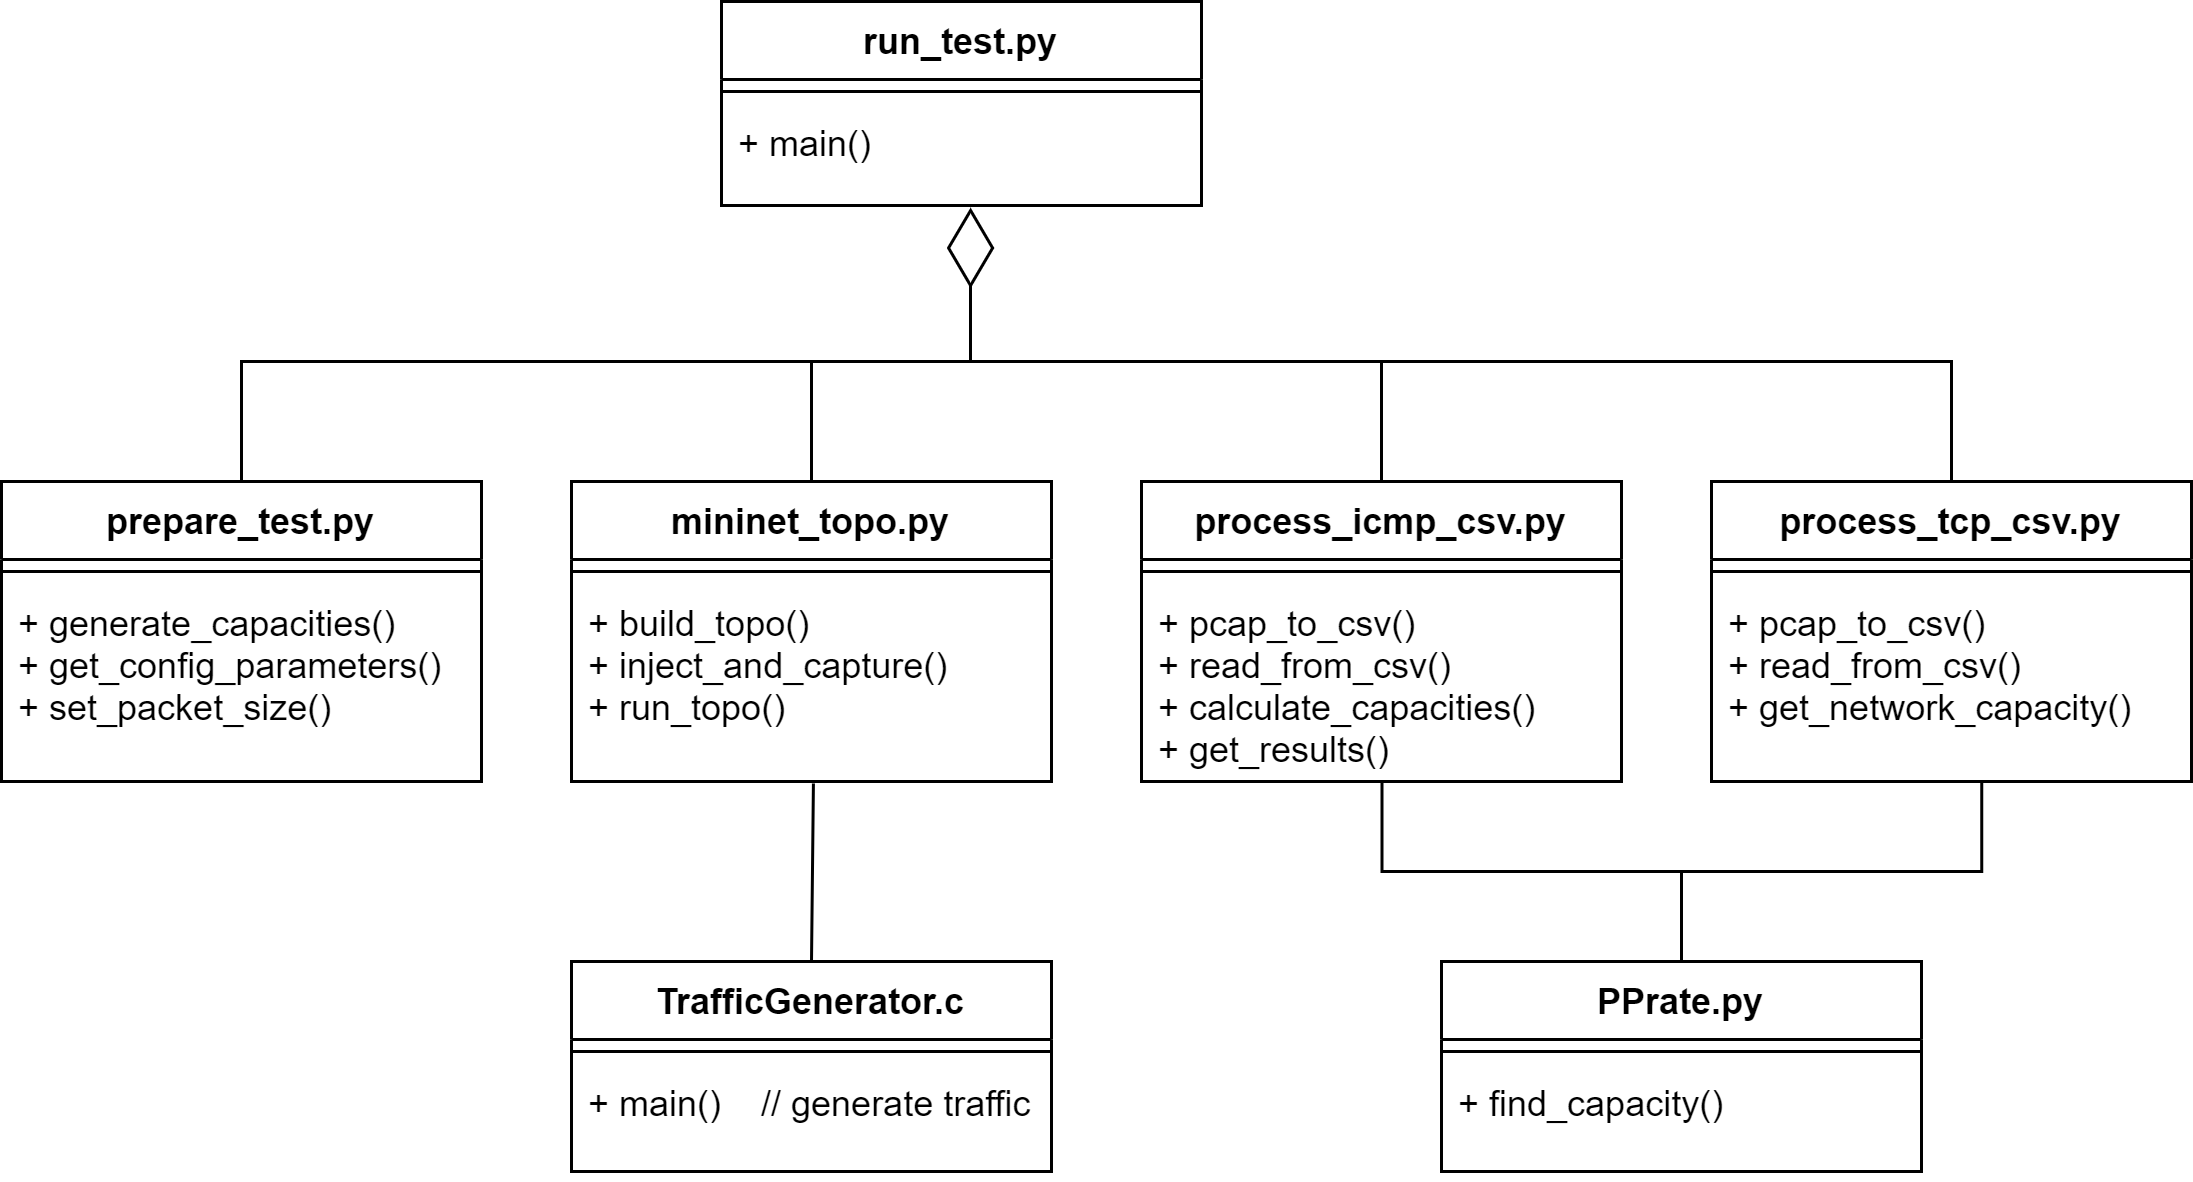
\includegraphics[width=\textwidth]{architecture}
 \caption{The architecture of the framework}
 \label{fig}

\end{figure}


\section{Setup}
In order to run the test measurements with our tool, several dependencies and software should be installed on the Linux machine.

The experiments conducted by us were run only on Mininet - a network emulator tool which creates a realistic virtual network of virtual hosts, switches, controllers and links and runs a real kernel and application code\cite{mnHome}.
To run the experiments on Mininet, it is necessary to install the emulator first.
It is highly recommended to install Mininet from the source GitHub repository instead of packages, as the Mininet homepage\cite{mnInstall} states that packages could give an older version. 

Mininet installation:
\begin{lstlisting}[language=bash]
  $ git clone git://github.com/mininet/mininet
  $ mininet/util/install.sh [options]
\end{lstlisting}
The default branch normally will install the latest stable version, however in case a user wishes to have any other version, it also possible to check out the branch with the following script before running \texttt{install.sh}:
\begin{lstlisting}[language=bash]
  $ cd mininet
  $ git tag  # list available versions
  $ git checkout -b mininet-2.3.0 2.3.0  # or any desired version from the list
  $ cd ..
\end{lstlisting}
\emph{Note that Mininet must run as a root.}


As for the rest, the following dependencies are required to be installed to run experiments:
\begin{itemize}
	\item pandas
	\item NumPy
	\item SciPy
	\item tshark
	\item iPerf
\end{itemize}
For setting up these and compiling the \texttt{TrafficGenerator.c} program, run \texttt{install.sh} script in the \texttt{ma-andguladze/App} directory.

\section{Running Tests}
The measurements must be run with a \texttt{JSON} config file containing all the parameters that are interesting and important for our measurements. Manipulating these parameters gives us a better picture about strengths and weaknesses of our approach.

The following script executes the experiment:
\begin{lstlisting}[language=bash]
  $ sudo python run_test.py <config file>
\end{lstlisting}

The following parameters must be passed to the program via the config file:
\begin{itemize}
	\item \texttt{topo\textunderscore size} - The number of routers between the source host and the destination host.
	\item \texttt{capacity\textunderscore range} - The range of numbers from which a capacity for each link will be generated
	\item \texttt{packet\textunderscore size} - The size of each packet (in bytes) that will be sent from the source host to the destination.
	\item \texttt{packets\textunderscore per\textunderscore hop} - The amount of packets that will be targeted at each hop
	\item \texttt{icmp\textunderscore ratelimit} - The artificial ICMP rate limit that will be assigned to each router. The default value is 0.
	\item \texttt{packet\textunderscore loss} - The artificial packet loss that will be assigned to each router. The default value is 0.
	\item \texttt{cross\textunderscore traffic} - The coefficient of the cross traffic load. The Optimal value is recommended to be assigned from 0 to 1.0, the value of 0 meaning an empty network without any cross traffic. 
\end{itemize}
%\acuseall
\printacronyms[heading=chapter,name=List of acronyms]

\clearpage
\pagestyle{thesischapter}

\cleardoublepage
\selectlanguage{english}
\printbibliography[heading=bibintoc]
%\begin{thebibliography}{9}
\bibitem{prasad}
Prasad et al. - Bandwidth estimation - metrics, measurement techniques, and tools 

\bibitem[brzoza]{brzoza}
Patryk Brzoza - Implementation and Evaluation of Passive Capacity Estimation (2019)

\bibitem{abut}
Fatih Abut. "Through the Diversity of Bandwidth-Related Metrics, Estimation Techniques and Tools An Overview". (2018)

\bibitem{pprate}
Taoufik En-Najjary, Guillaume Urvoy-Keller. "PPrate: A passive capacity estimation tool" (2006)

\bibitem{pathrate}
Constantinos Dovrolis et al. - Packet-Dispersion Techniques and a Capacity-Estimation Methodology (2004)

\bibitem{rawsocks}
"How to Code Raw Sockets in C on Linux" URL: \url{https://www.binarytides.com/raw-sockets-c-code-linux/}

\bibitem{lamport94}
Leslie Lamport (1994) \emph{\LaTeX: a document preparation system}, Addison
Wesley, Massachusetts, 2nd ed.
\end{thebibliography}


%\cleardoublepage
\clearpage
\pagestyle{empty}
%\mbox{}
%\clearpage

\end{document}


